\documentclass[11pt,a4paper]{article}
\usepackage[margin=22mm]{geometry}
\usepackage{graphicx}
\usepackage{booktabs}
\usepackage{hyperref}
\hypersetup{hidelinks}
\usepackage{microtype}
\usepackage{caption}
\captionsetup{font=small}
\graphicspath{{figures/}}
\title{What Code LLMs Learn: Results Across Four Programming Languages}
\author{Comparative extension of Anand et al.'s results}
\date{15 September 2026}

\begin{document}
\maketitle

\section{Results: Python, Java, JavaScript, and Go}

This section extends Section~4 of Anand et al., \emph{A Critical Study of What Code-LLMs (Do Not) Learn}, from Python to Java, JavaScript, and Go. We retain the paper's organization: attention-based AST/DFG overlap and graph-edit distance (GED), followed by qualitative t-SNE and DirectProbe analysis of hidden representations. Figures~\ref{fig:recall} and \ref{fig:ged} are counterparts to the paper's Figures~4 and 5; Figures~\ref{fig:token-tsne} and \ref{fig:distance-tsne} correspond to its Appendix Figures~10 and 11; Tables~\ref{tab:distance}--\ref{tab:dfg} correspond to its Tables~1--3. A counterpart to its Appendix Figure~7 (precision) is included in Figure~\ref{fig:precision}.

The six-model attention-overlap cohort comprises CodeBERT, GraphCodeBERT, UniXcoder, PLBART, CodeT5, and CodeT5+220M. The multilingual GED and DirectProbe schedules were deliberately restricted to CodeBERT, GraphCodeBERT, and CodeT5; no GED or probing curves for the other three models are implied. The paper also studied larger and fine-tuned models that have \emph{not} been run on the three new languages, so its conclusions about model scale or fine-tuning are outside the scope of this comparison. For recall and precision we use the project's final-3000 results for all four languages. For GED and DirectProbe, Python uses the original paper-repository output; Java, JavaScript, and Go use the project's completed final-3000 runs. The Python GED therefore has a different run provenance and potentially a different NetworkX version; numeric cross-language differences should be read as descriptive, not a controlled effect of language alone.

\subsection{Attention analysis}

\paragraph{AST and data-flow overlap.} Figure~\ref{fig:recall} shows the recall of each layer's best-F-score attention head against AST and DFG relations, using the paper's 0.05 threshold. Across the six models, the median of each model's peak AST recall is 0.363 for Python, 0.350 for Java, 0.345 for JavaScript, and 0.363 for Go. This preserves the paper's principal observation that only a minority of syntactic relations are recovered by the selected attention graphs; there is no consistent gain in AST recall merely from changing programming language. The paper's ``30--40\%'' is an approximate characterization, not a strict ceiling: PLBART's peak AST recall ranges from 0.416 (Java) to 0.462 (Go). The equivalent median peak DFG recall is 0.559, 0.710, 0.610, and 0.595, respectively. Java's DFG recall is notably higher than the Python reference in this corpus, so the paper's ``around 50\%'' description is not a four-language upper bound. This is a corpus- and evaluation-specific finding, not evidence that Java is intrinsically easier for the models.

\begin{figure}[p]
\centering
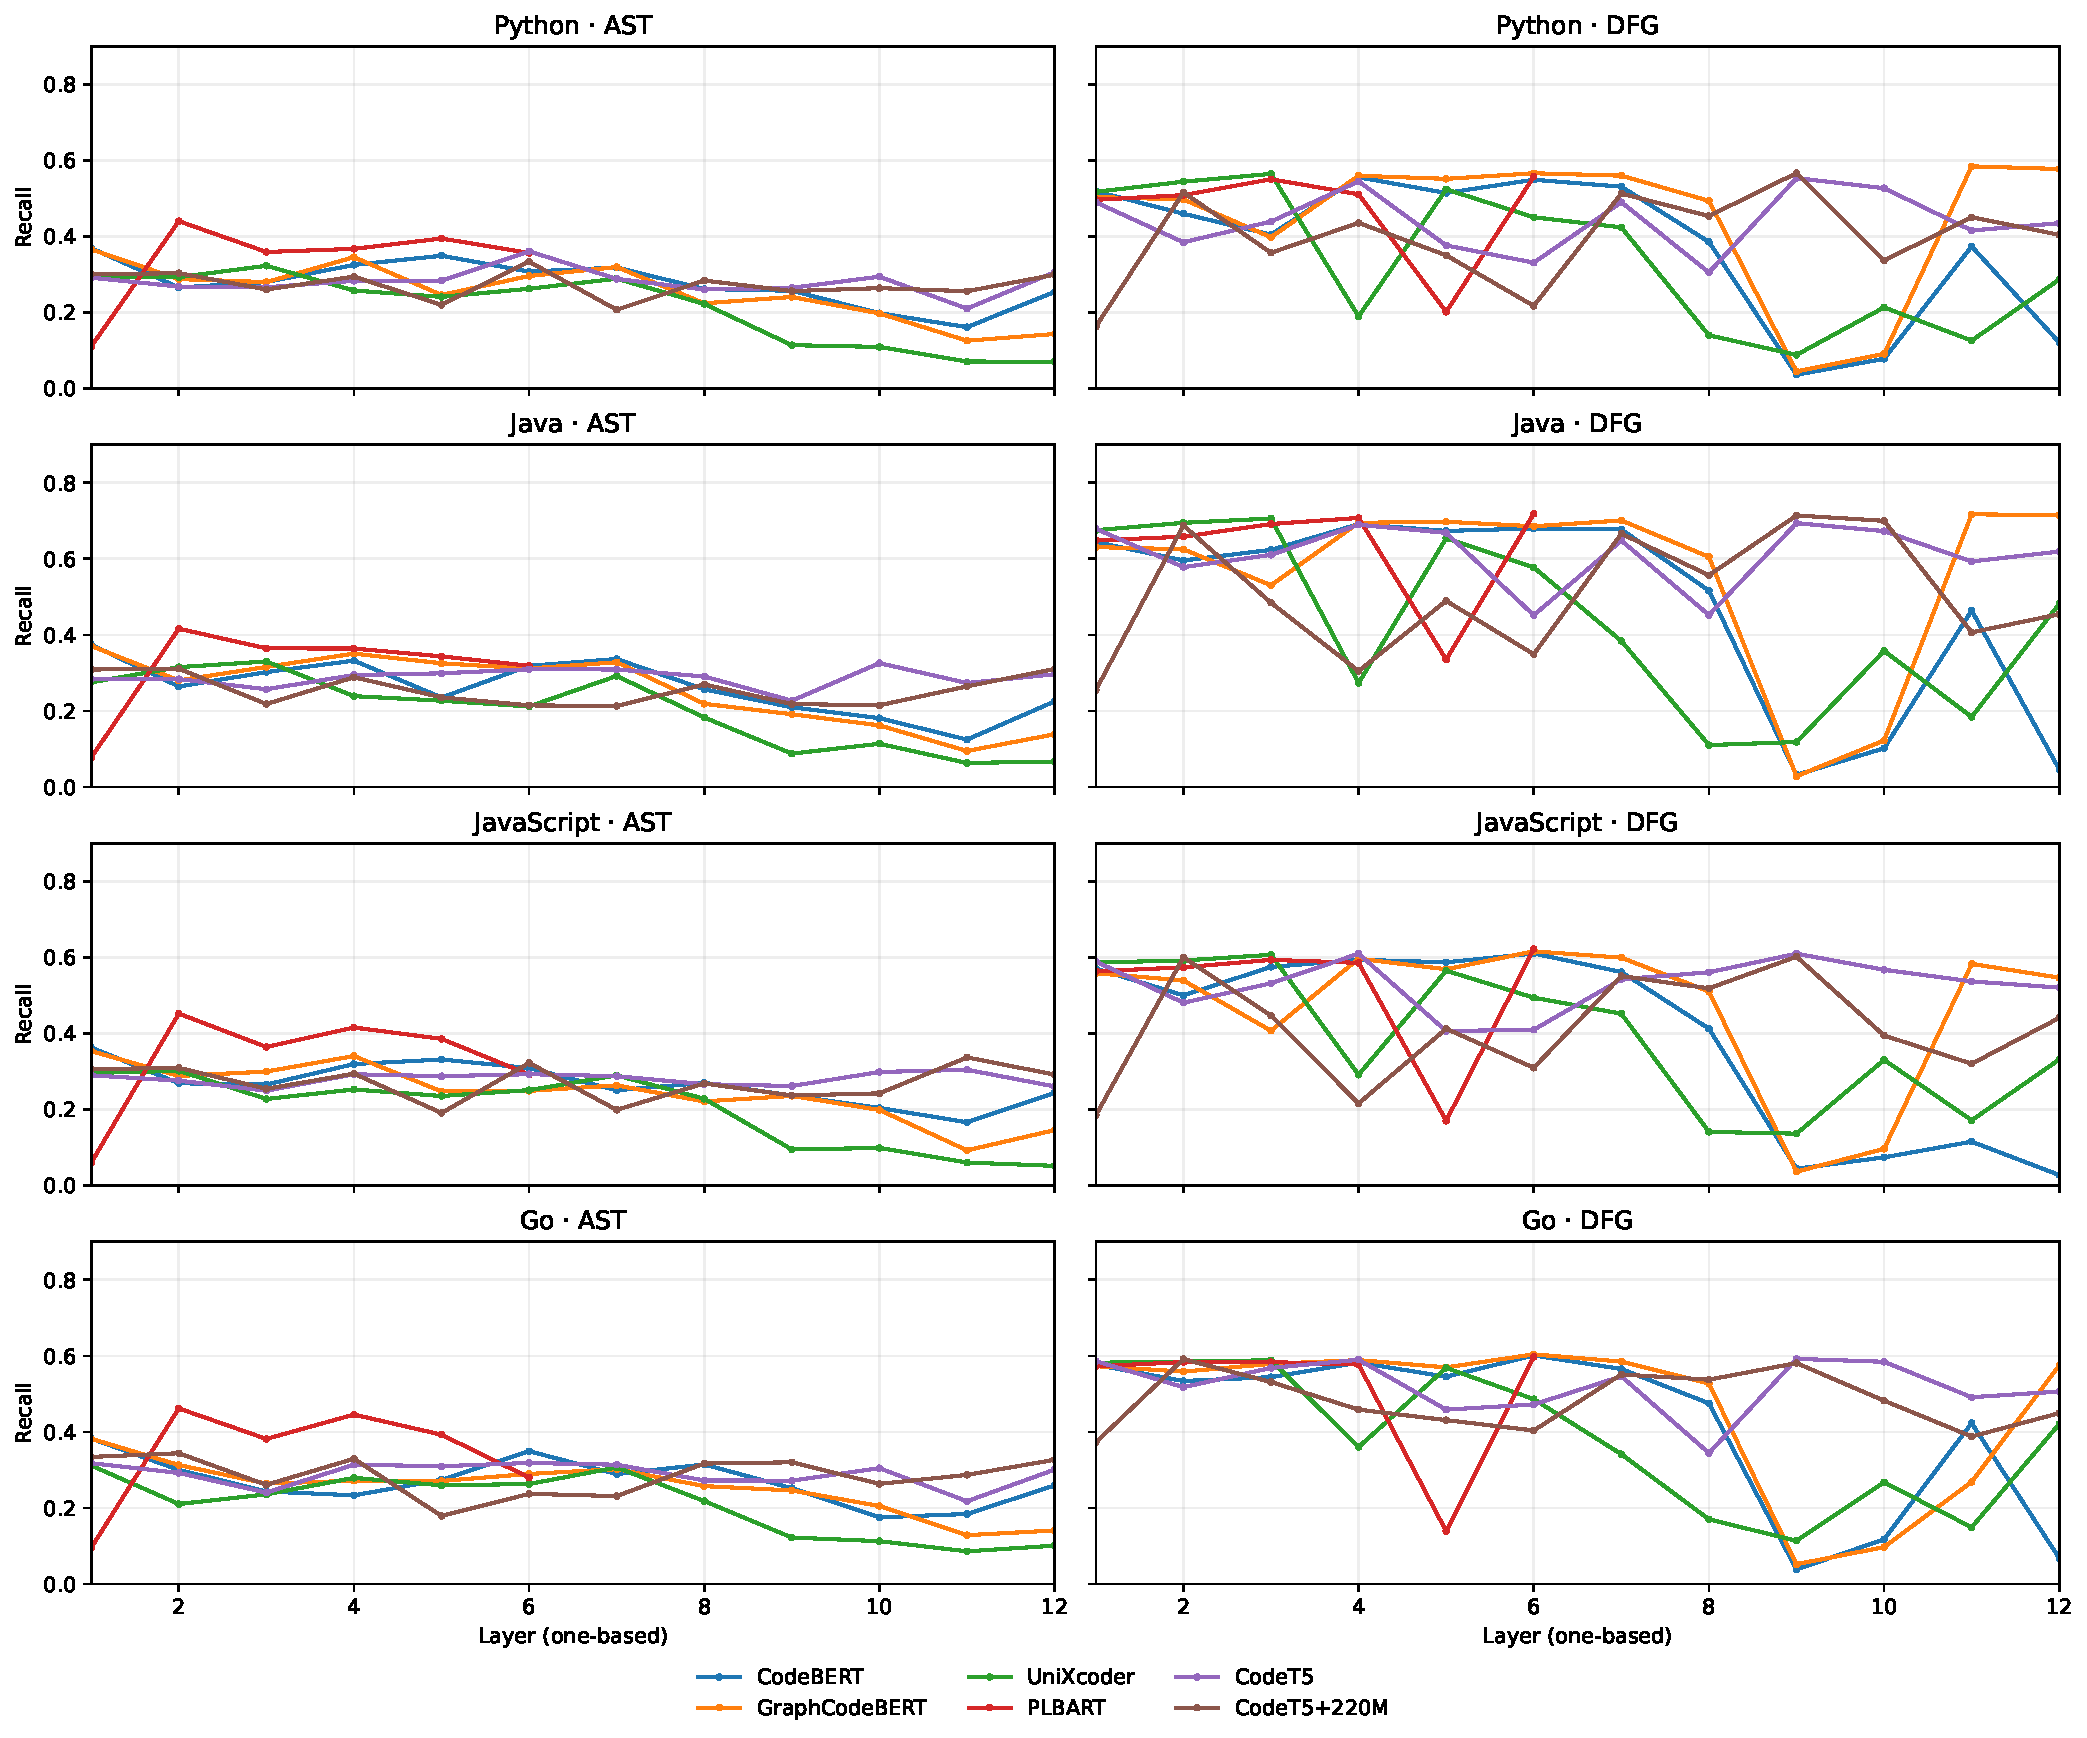
\includegraphics[width=\textwidth,height=0.82\textheight,keepaspectratio]{figures/figure4_recall_four_languages.pdf}
\caption{Four-language counterpart to the paper's Figure~4: recall of selected attention graphs against AST (left) and DFG (right), by layer. Each panel contains the six available models; PLBART has six layers. Python and the additional languages use final-3000 recomputations.}
\label{fig:recall}
\end{figure}

Higher recall does not by itself imply accurate relation selection. The precision counterpart in Figure~\ref{fig:precision} shows that median peak DFG precision across the six models is only 0.154, 0.095, 0.113, and 0.103 for Python, Java, JavaScript, and Go, respectively. Thus Java's high DFG recall is paired with low DFG precision. The attention results continue to indicate incomplete and noisy relation encoding, while differing in the exact recall--precision trade-off by language and model.

An audit of the matched 3,000-program GraphCodeBERT DFGs also finds unequal ground-truth density: mean directed-edge density is 0.005254 in Python, 0.002501 in Java, 0.003585 in Go, and 0.002896 in JavaScript. A controlled four-language toy example yields the same binary dependencies, but the extractor's signed relation labels differ by language; thus the DFG recall differences may partly reflect graph sparsity and native label conventions, not just representation quality. Separately, PLBART's recomputed Python AST-recall curve differs from the stored paper reference by a mean absolute 0.03755, despite complete 3,000-program coverage. All-head and deterministic-inference checks do not resolve the discrepancy. We therefore treat PLBART's absolute cross-language overlap levels as exploratory; the other five models reproduce the Python reference much more closely. The checks and raw results are documented in the accompanying validation audit.

\paragraph{Graph-edit distance.} Figure~\ref{fig:ged} plots each layer's minimum GED per node across attention heads for complete AST, AST without identifiers, and DFG, following the paper's Figure~5 layout. For all four languages and all three evaluated models, DFG is generally the nearest of the three code graphs to the selected attention graph. The complete AST is much farther than the non-identifier AST. Taking the median across models of each model's best-layer distance, complete-AST GED is 3.110, 3.162, 2.996, and 2.519 for Python, Java, JavaScript, and Go; the non-identifier AST values are 1.399, 1.450, 1.606, and 1.202. The gap is approximately 1.9--2.2-fold at this summary level. This extends the paper's evidence that edges connecting syntactic tokens with identifiers are poorly represented in attention graphs. As in the paper, GED is normalized per node; it is not an absolute count of missed edges. Since graphs, program lengths, parser labels, and Python GED provenance differ, these numbers should not be interpreted as a causal ranking of language quality.

\begin{figure}[p]
\centering
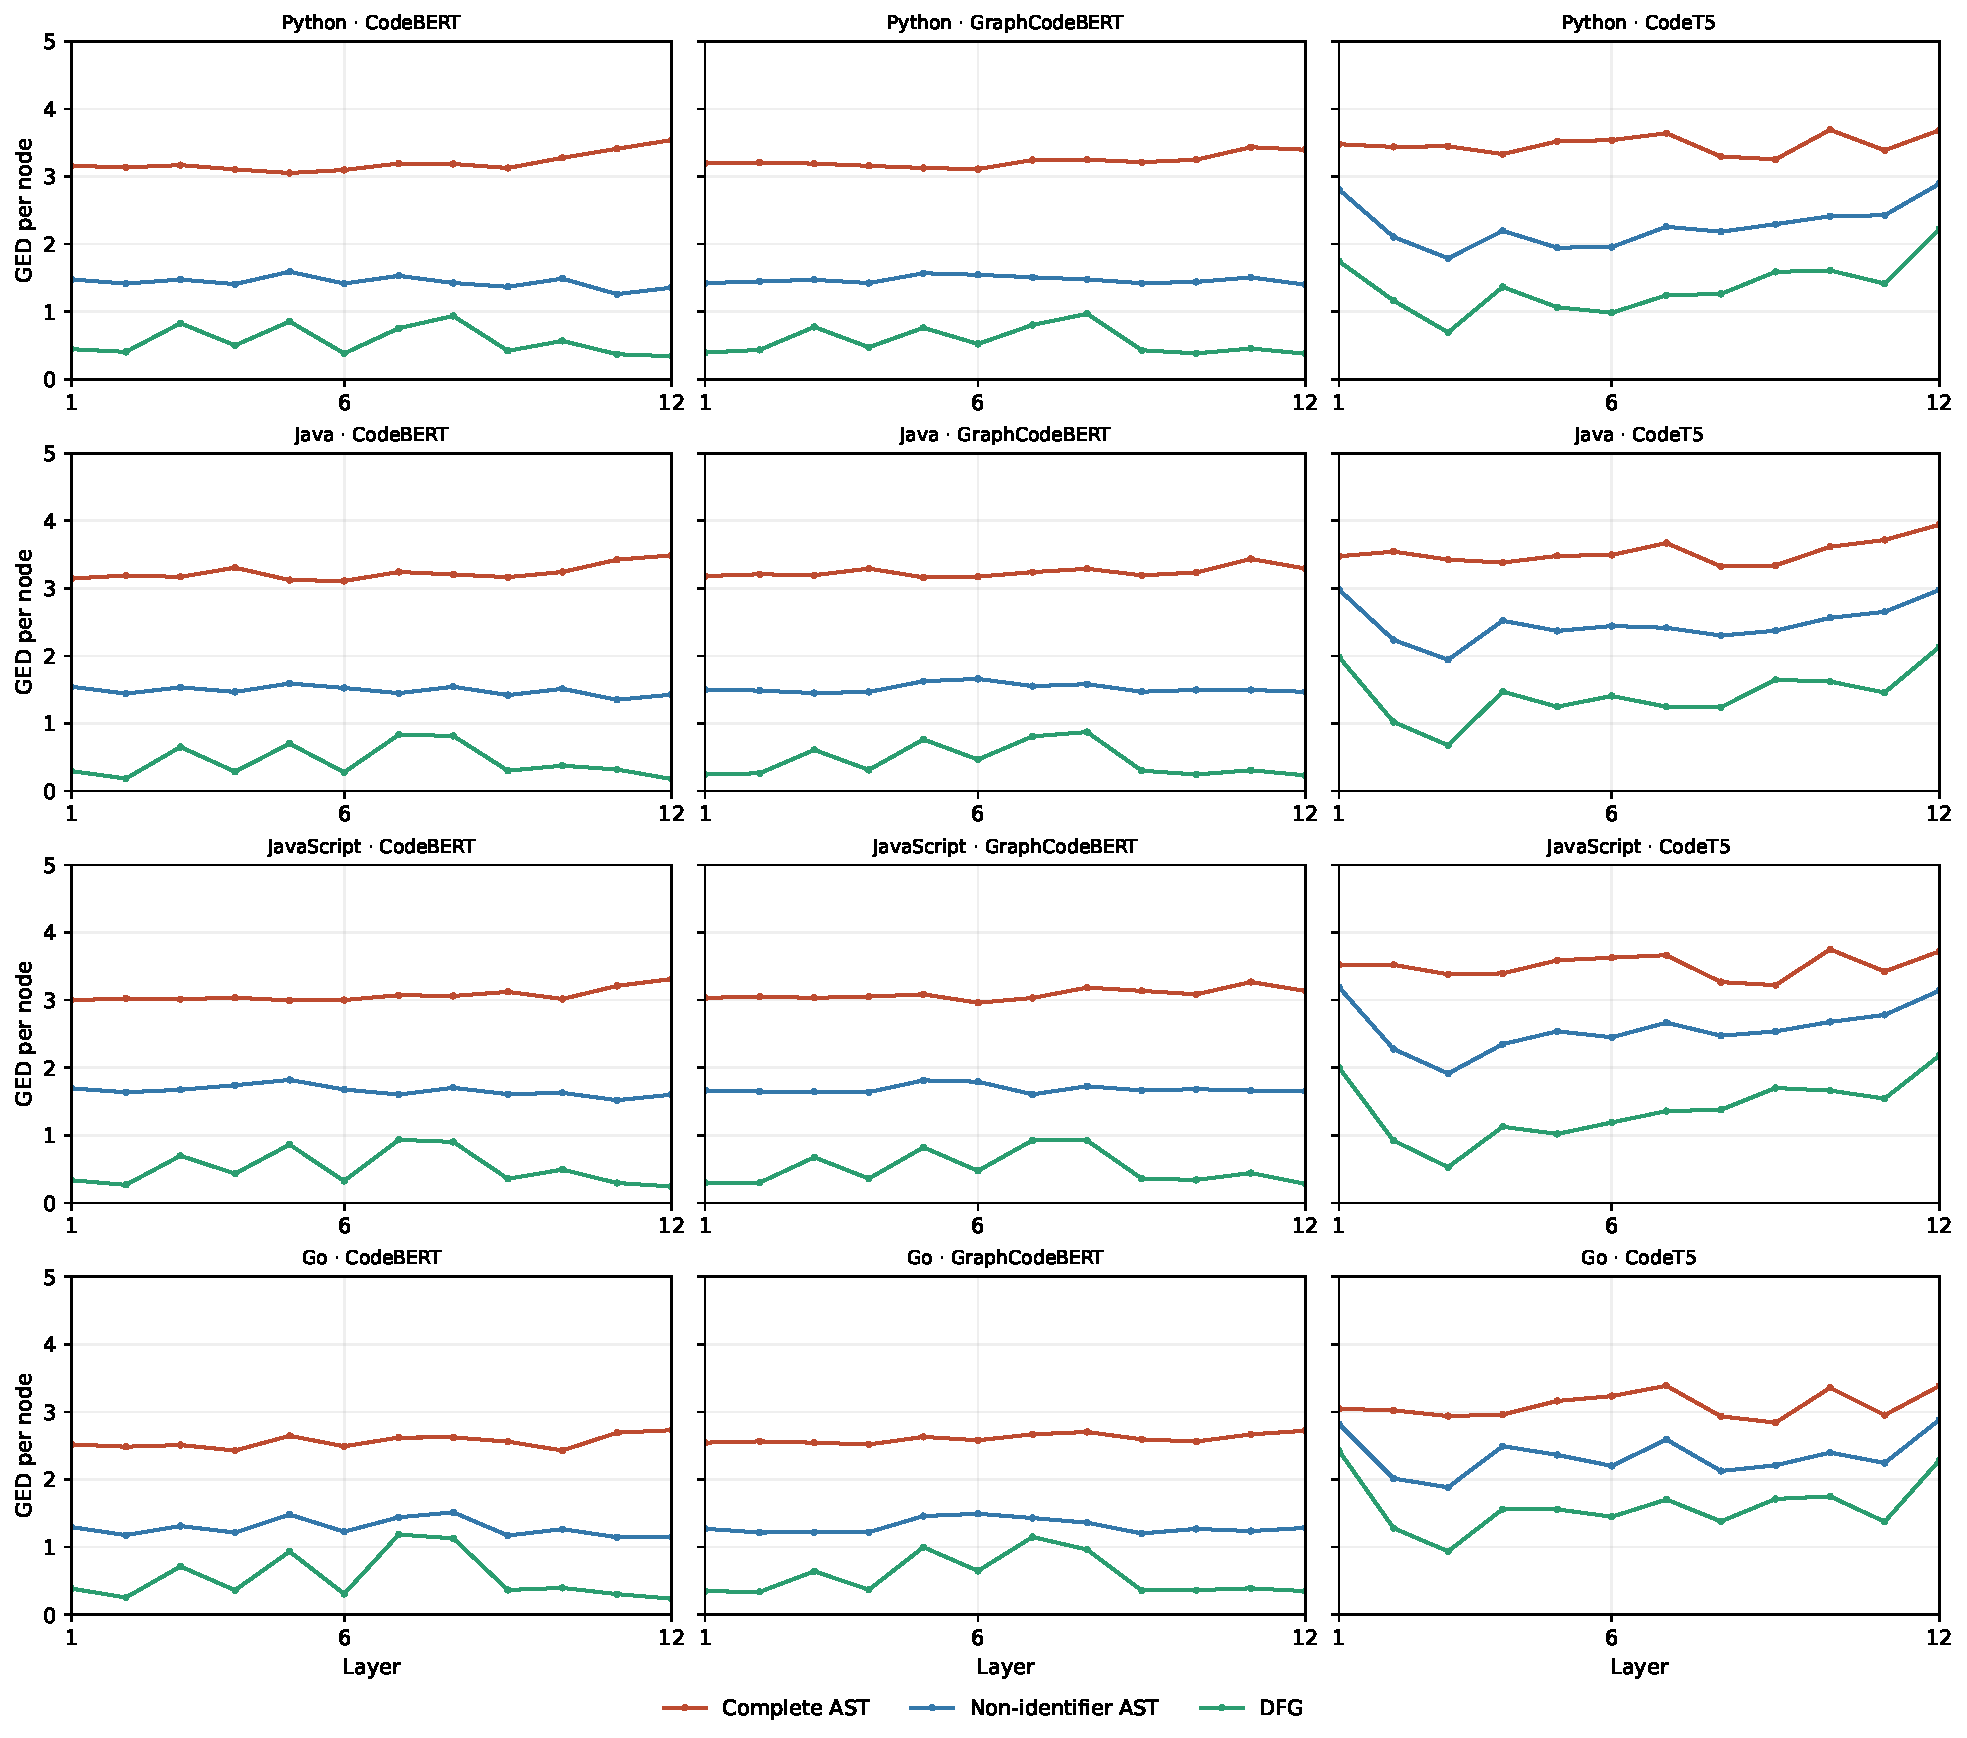
\includegraphics[width=\textwidth,height=0.82\textheight,keepaspectratio]{figures/figure5_ged_four_languages.pdf}
\caption{Four-language counterpart to the paper's Figure~5: lower GED per node means greater graph similarity. Only CodeBERT, GraphCodeBERT, and CodeT5 were scheduled for GED on all four languages. Python curves use paper-repository reference JSON; the others use validated multilingual legacy-GED outputs.}
\label{fig:ged}
\end{figure}

\subsection{Analysis of hidden representations}

\paragraph{Qualitative visualization.} Figure~\ref{fig:token-tsne} compares layer-5 CodeBERT token-type t-SNE plots for all four languages. Token classes and common lexical forms visibly contribute to the geometry, consistent with the paper's Figure~10 and its conclusion that the projection is not organized simply by AST relations. Figure~\ref{fig:distance-tsne} pairs an AST-distance projection and a hidden-representation projection for a selected program in each language, paralleling the paper's Figure~11. The underlying rank correlation between AST and hidden distances for these selected programs is weak: Spearman's $r$ is 0.167 (Python), 0.142 (Java), 0.245 (JavaScript), and 0.186 (Go). JavaScript is the highest here, but none approaches a strong monotonic correspondence. These plots are qualitative illustrations: each language uses a different set of programs and, for the distance plot, a different selected program; independently fitted t-SNE coordinates cannot be aligned or compared numerically across panels. The paper's Figure~11 uses its specific Python example in Figure~6a, whereas these are final-3000 project visualizations.

\begin{figure}[p]
\centering
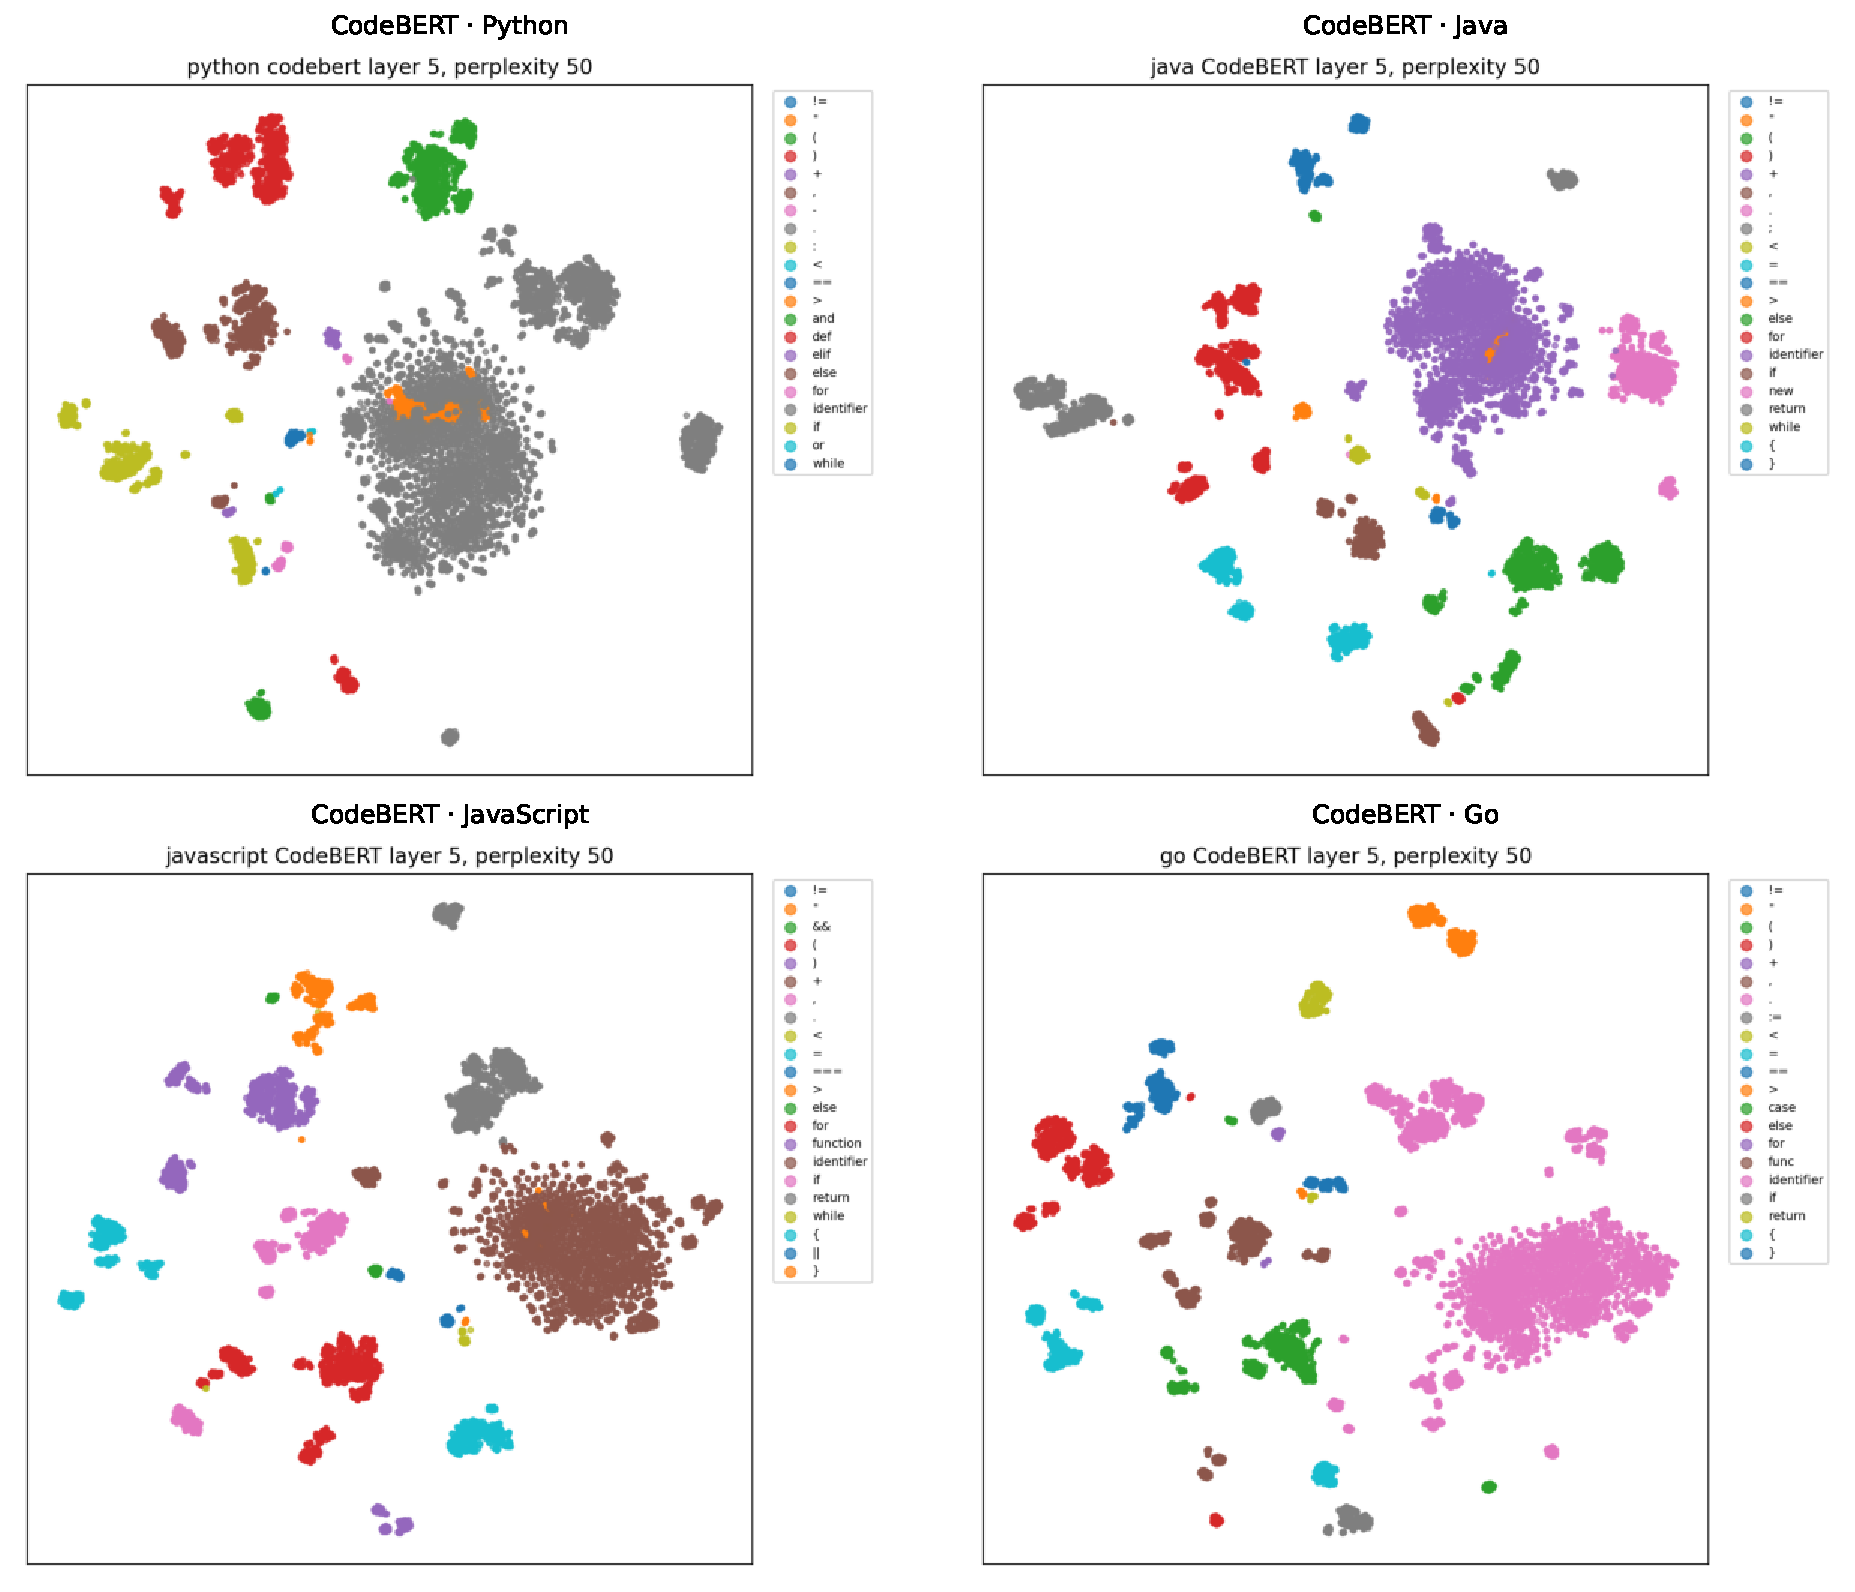
\includegraphics[width=\textwidth,height=0.82\textheight,keepaspectratio]{figures/figure10_token_tsne_four_languages.pdf}
\caption{Four-language counterpart to the paper's Figure~10: CodeBERT layer-5 token-type t-SNE. Each language uses up to 100 eligible programs selected from its final-3000 sample; lexical categories are language-specific.}
\label{fig:token-tsne}
\end{figure}

\begin{figure}[p]
\centering
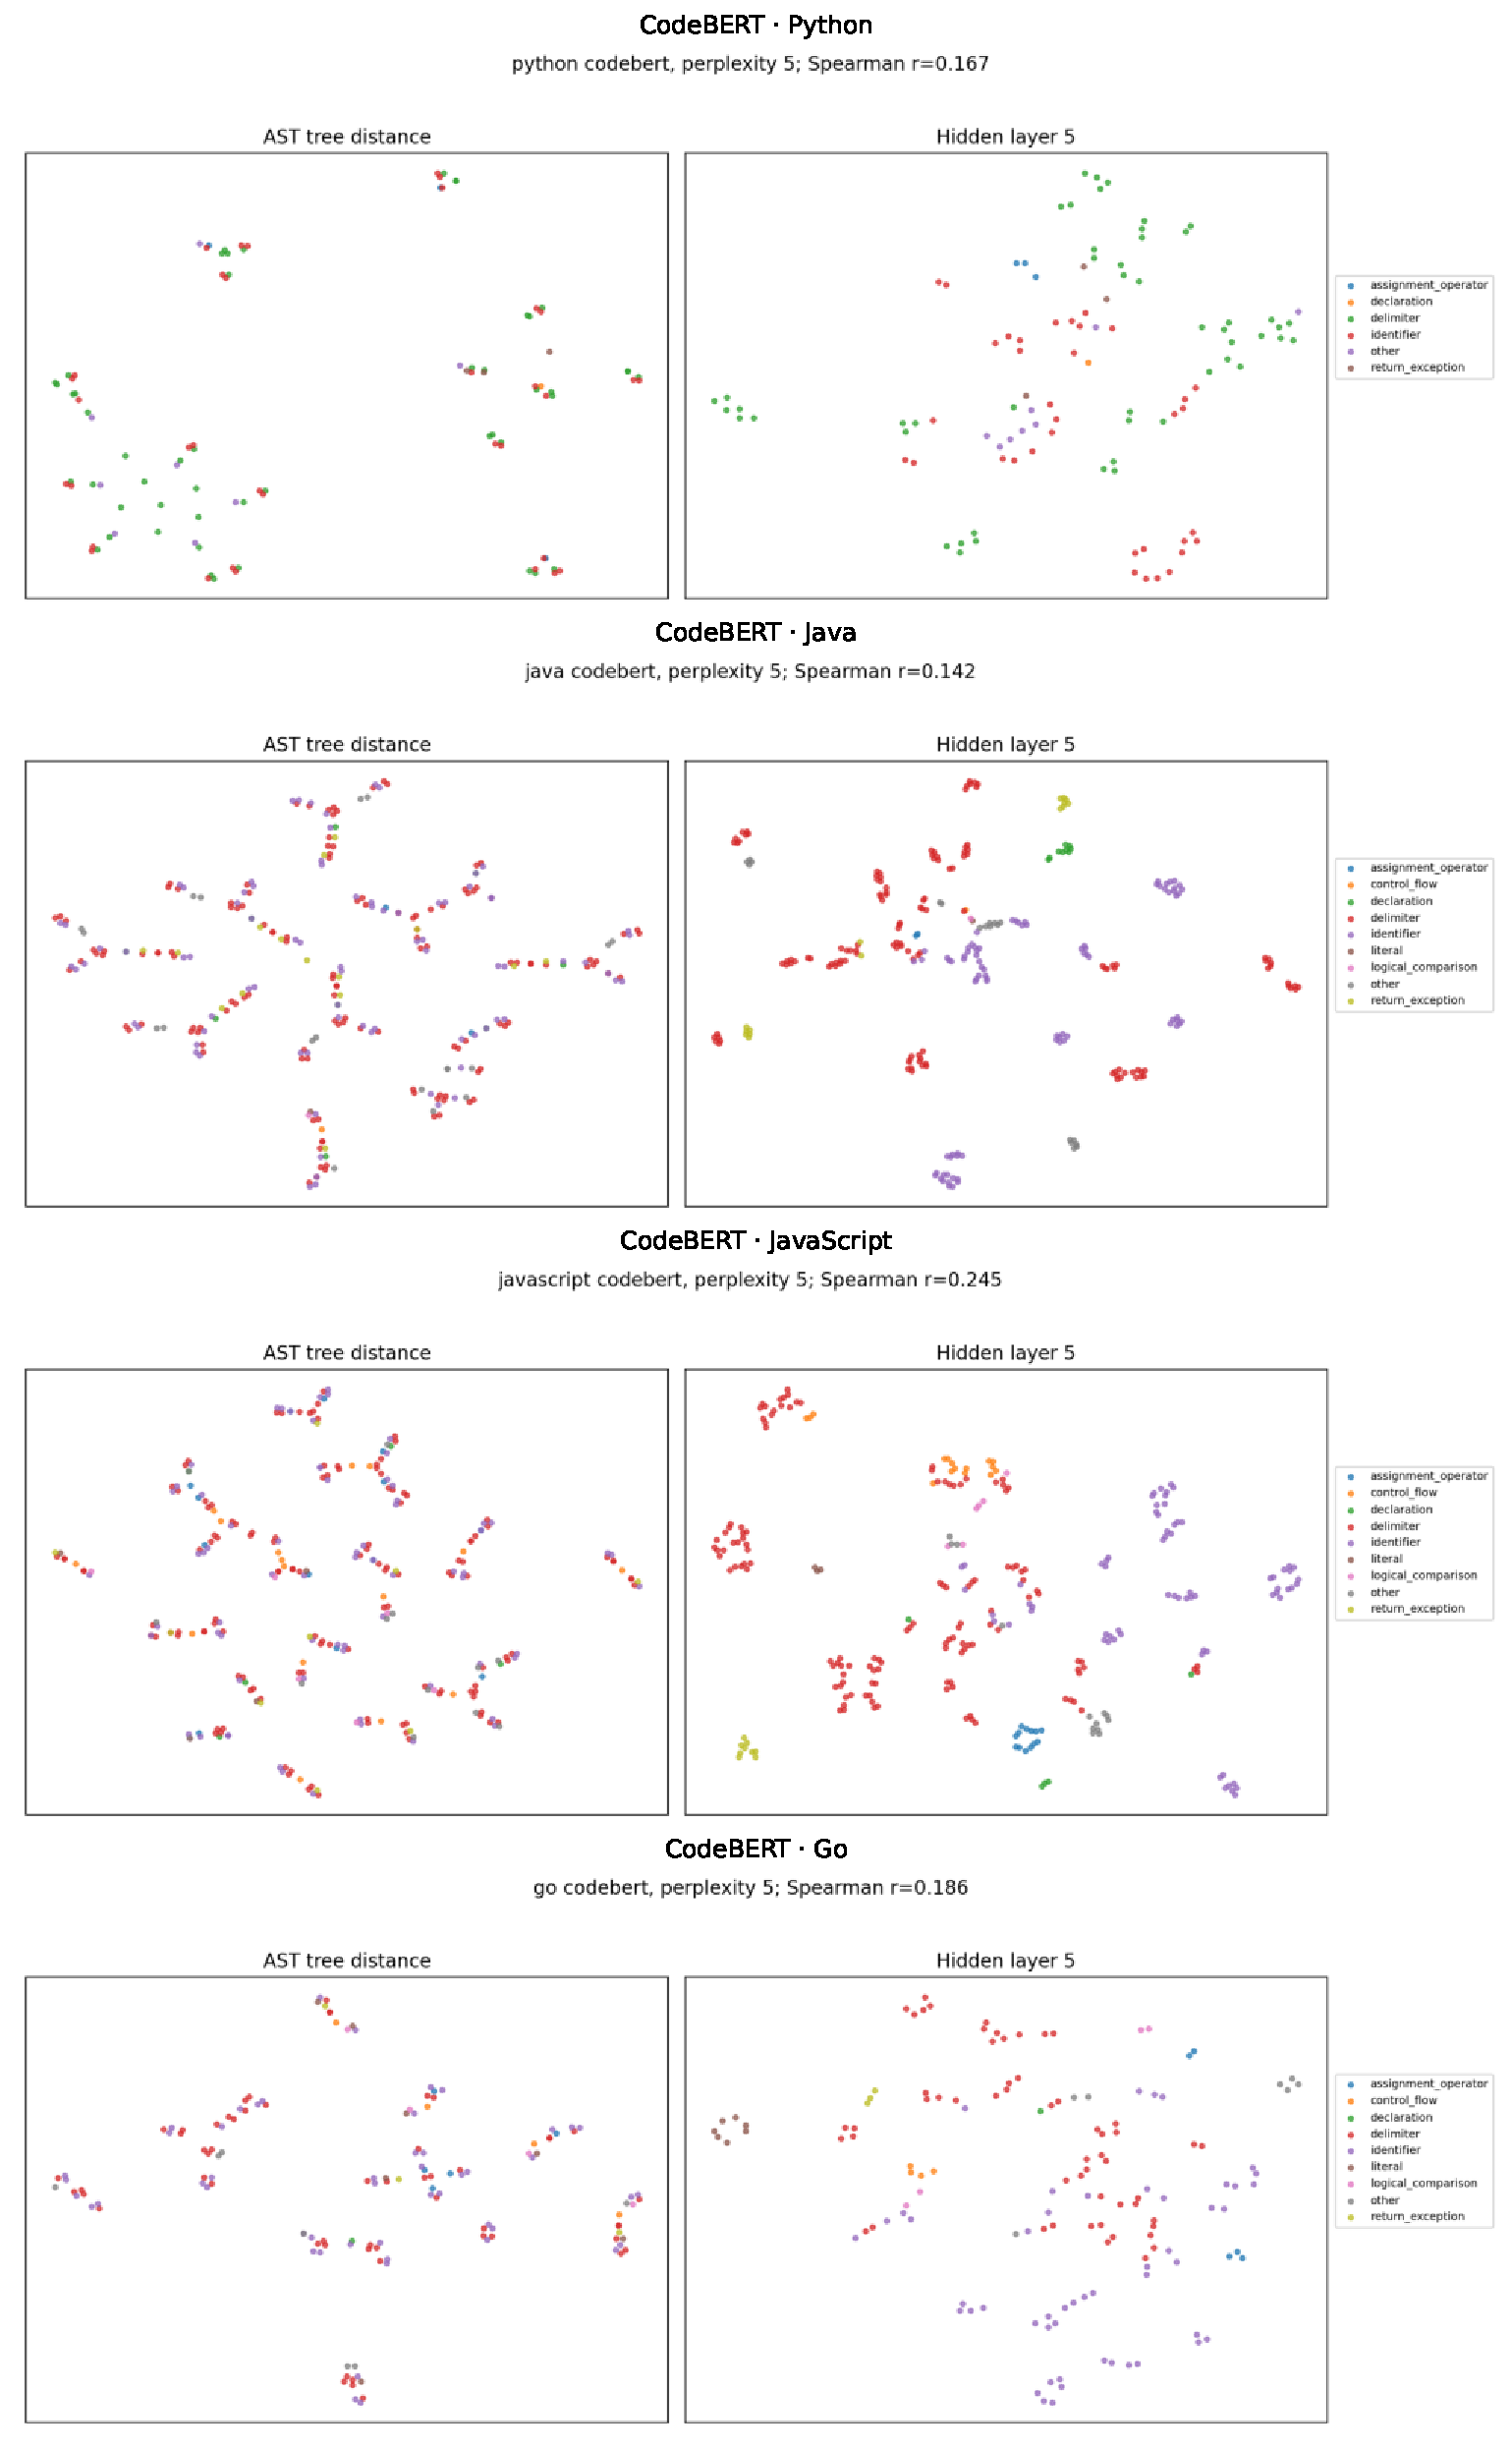
\includegraphics[width=\textwidth,height=0.82\textheight,keepaspectratio]{figures/figure11_distance_tsne_four_languages.pdf}
\caption{Four-language counterpart to the paper's Figure~11: AST-distance (left within each subpanel) versus CodeBERT hidden-distance (right) t-SNE for a selected program at layer 5 and perplexity 5. The specimens are different across languages.}
\label{fig:distance-tsne}
\end{figure}

\paragraph{DirectProbe.} Tables~\ref{tab:distance}--\ref{tab:dfg} report the number of clusters and test accuracy for every paper task in the three-model multilingual schedule, using the paper's last-layer convention (layer 12). Python's GraphCodeBERT and CodeT5 values reproduce the corresponding rows of the paper's Tables~1--3 from the original output files; CodeBERT reference rows, available in the paper repository and appendix, are included as well. Each AST-distance task has 1,300 test pairs, each sibling task 600, and the DFG task 900. Per-label accuracies are preferable to a single pooled score because the five distance labels and three DFG labels differ substantially in difficulty.

For keyword--all AST distance, cluster counts are 9--14 across the four languages for only five labels. Accuracy generally falls as distance grows, but the shape is not universal: Java has especially weak distance-4 accuracy (0.43--0.52 for the three models), whereas Go is stronger at distance 2 (0.90--0.93). Keyword--identifier distance is not uniformly harder in the added languages: median three-model overall accuracy is 0.610 for Python but 0.683 for Java, 0.660 for JavaScript, and 0.771 for Go. This moderates the paper's Python-specific statement that this task is always poorer than keyword--all distance. It does \emph{not} imply that identifier relations are completely encoded; the cluster counts and per-label variation remain substantial.

Sibling prediction is comparatively accurate. Median three-model overall accuracy on keyword--all pairs is 0.867 (Python), 0.847 (Java), 0.805 (JavaScript), and 0.882 (Go); keyword--identifier siblings are 0.825, 0.762, 0.770, and 0.867. For DFG edges the medians are 0.836, 0.868, 0.861, and 0.903. The no-edge class is typically less accurate than positive comes-from and computed-from classes, as in the paper's Table~3. Contrary to a literal extension of the paper's ``usually twice as many clusters as labels'' wording, some added-language DFG runs form exactly three clusters for three labels, while the AST-distance runs form substantially more than five. The results support nontrivial and task-dependent geometry, but cluster count alone cannot establish a general absence of \emph{linear} decodability. DirectProbe's cluster count is a property of its data split, embeddings, solver, and clustering procedure.

The new-language DirectProbe data were split by token pair rather than source program: the median fraction of test programs also occurring in training is 98.96\% across the 45 layer-12 configurations. A separate standardized linear-probe control, using the existing features and five program-disjoint folds per configuration, drops below its pair-split score in 35/45 cases (median 1.76 percentage points), including all nine DFG cases (median 4.37 points). This does \emph{not} measure how much the original Gurobi-based DirectProbe scores would change, but it makes the existing per-label tables split-sensitive. Moreover, the signed DFG classes are native to each language's extractor, so per-class comparisons are not semantically identical across languages. Program-disjoint DirectProbe reruns with controlled label definitions are needed before making stronger cross-language claims.

\begin{table}[p]
\centering
\small
\resizebox{\textwidth}{!}{%
\begin{tabular}{llrrrrrr}
\toprule
\multicolumn{8}{l}{Keyword--all AST distance} \\
Language & Model & Clusters & 2 & 3 & 4 & 5 & 6 \\
\midrule
Python & CodeBERT & 10 & 0.85 & 0.75 & 0.73 & 0.68 & 0.55 \\
Python & GraphCodeBERT & 9 & 0.84 & 0.78 & 0.67 & 0.67 & 0.57 \\
Python & CodeT5 & 10 & 0.83 & 0.79 & 0.70 & 0.64 & 0.60 \\
\addlinespace
Java & CodeBERT & 9 & 0.90 & 0.77 & 0.45 & 0.58 & 0.61 \\
Java & GraphCodeBERT & 10 & 0.91 & 0.67 & 0.52 & 0.59 & 0.48 \\
Java & CodeT5 & 14 & 0.90 & 0.63 & 0.43 & 0.58 & 0.51 \\
\addlinespace
JavaScript & CodeBERT & 9 & 0.85 & 0.81 & 0.77 & 0.65 & 0.52 \\
JavaScript & GraphCodeBERT & 9 & 0.89 & 0.77 & 0.64 & 0.71 & 0.47 \\
JavaScript & CodeT5 & 10 & 0.90 & 0.68 & 0.63 & 0.64 & 0.52 \\
\addlinespace
Go & CodeBERT & 12 & 0.92 & 0.78 & 0.63 & 0.68 & 0.56 \\
Go & GraphCodeBERT & 10 & 0.90 & 0.80 & 0.70 & 0.66 & 0.62 \\
Go & CodeT5 & 10 & 0.93 & 0.78 & 0.71 & 0.65 & 0.70 \\
\addlinespace
\midrule
\multicolumn{8}{l}{Keyword--identifier AST distance} \\
Language & Model & Clusters & 2 & 3 & 4 & 5 & 6 \\
\midrule
Python & CodeBERT & 7 & 0.82 & 0.66 & 0.56 & 0.53 & 0.51 \\
Python & GraphCodeBERT & 7 & 0.79 & 0.68 & 0.52 & 0.57 & 0.49 \\
Python & CodeT5 & 6 & 0.78 & 0.66 & 0.59 & 0.55 & 0.48 \\
\addlinespace
Java & CodeBERT & 8 & 0.92 & 0.80 & 0.58 & 0.54 & 0.55 \\
Java & GraphCodeBERT & 7 & 0.87 & 0.81 & 0.60 & 0.62 & 0.52 \\
Java & CodeT5 & 5 & 0.85 & 0.82 & 0.62 & 0.65 & 0.50 \\
\addlinespace
JavaScript & CodeBERT & 5 & 0.90 & 0.73 & 0.61 & 0.57 & 0.60 \\
JavaScript & GraphCodeBERT & 5 & 0.84 & 0.72 & 0.56 & 0.53 & 0.53 \\
JavaScript & CodeT5 & 5 & 0.85 & 0.73 & 0.63 & 0.52 & 0.57 \\
\addlinespace
Go & CodeBERT & 5 & 0.91 & 0.80 & 0.80 & 0.70 & 0.64 \\
Go & GraphCodeBERT & 5 & 0.93 & 0.78 & 0.71 & 0.67 & 0.61 \\
Go & CodeT5 & 5 & 0.94 & 0.81 & 0.76 & 0.72 & 0.68 \\
\addlinespace
\bottomrule
\end{tabular}%
}
\caption{Four-language DirectProbe AST tree-distance results at layer 12. Values are per-label test accuracy; Python is the paper-repository reference and the other languages are final-3000 runs.}
\label{tab:distance}
\end{table}

\begin{table}[p]
\centering
\small
\resizebox{\textwidth}{!}{%
\begin{tabular}{llrrr}
\toprule
\multicolumn{5}{l}{Keyword--all siblings} \\
Language & Model & Clusters & Not siblings & Siblings \\
\midrule
Python & CodeBERT & 3 & 0.87 & 0.88 \\
Python & GraphCodeBERT & 4 & 0.76 & 0.87 \\
Python & CodeT5 & 7 & 0.82 & 0.91 \\
\addlinespace
Java & CodeBERT & 4 & 0.77 & 0.92 \\
Java & GraphCodeBERT & 4 & 0.83 & 0.89 \\
Java & CodeT5 & 4 & 0.76 & 0.90 \\
\addlinespace
JavaScript & CodeBERT & 4 & 0.79 & 0.89 \\
JavaScript & GraphCodeBERT & 4 & 0.76 & 0.85 \\
JavaScript & CodeT5 & 3 & 0.67 & 0.88 \\
\addlinespace
Go & CodeBERT & 4 & 0.86 & 0.90 \\
Go & GraphCodeBERT & 4 & 0.85 & 0.89 \\
Go & CodeT5 & 4 & 0.86 & 0.92 \\
\addlinespace
\midrule
\multicolumn{5}{l}{Keyword--identifier siblings} \\
Language & Model & Clusters & Not siblings & Siblings \\
\midrule
Python & CodeBERT & 4 & 0.79 & 0.87 \\
Python & GraphCodeBERT & 3 & 0.75 & 0.86 \\
Python & CodeT5 & 4 & 0.80 & 0.86 \\
\addlinespace
Java & CodeBERT & 4 & 0.70 & 0.82 \\
Java & GraphCodeBERT & 4 & 0.70 & 0.80 \\
Java & CodeT5 & 4 & 0.70 & 0.83 \\
\addlinespace
JavaScript & CodeBERT & 3 & 0.73 & 0.87 \\
JavaScript & GraphCodeBERT & 4 & 0.73 & 0.81 \\
JavaScript & CodeT5 & 5 & 0.71 & 0.79 \\
\addlinespace
Go & CodeBERT & 4 & 0.85 & 0.89 \\
Go & GraphCodeBERT & 4 & 0.79 & 0.84 \\
Go & CodeT5 & 4 & 0.84 & 0.91 \\
\addlinespace
\bottomrule
\end{tabular}%
}
\caption{Four-language DirectProbe AST-sibling results at layer 12. Values are per-label test accuracy.}
\label{tab:siblings}
\end{table}

\begin{table}[p]
\centering
\small
\resizebox{\textwidth}{!}{%
\begin{tabular}{llrrrr}
\toprule
\multicolumn{6}{l}{Identifier--identifier DFG} \\
Language & Model & Clusters & No edge & Comes from & Computed from \\
\midrule
Python & CodeBERT & 4 & 0.69 & 0.91 & 0.90 \\
Python & GraphCodeBERT & 7 & 0.71 & 0.94 & 0.93 \\
Python & CodeT5 & 4 & 0.57 & 0.86 & 0.90 \\
\addlinespace
Java & CodeBERT & 3 & 0.80 & 0.88 & 0.93 \\
Java & GraphCodeBERT & 3 & 0.85 & 0.85 & 0.97 \\
Java & CodeT5 & 3 & 0.76 & 0.85 & 0.96 \\
\addlinespace
JavaScript & CodeBERT & 3 & 0.77 & 0.91 & 0.96 \\
JavaScript & GraphCodeBERT & 4 & 0.78 & 0.89 & 0.91 \\
JavaScript & CodeT5 & 5 & 0.69 & 0.84 & 0.95 \\
\addlinespace
Go & CodeBERT & 3 & 0.82 & 0.95 & 0.96 \\
Go & GraphCodeBERT & 4 & 0.78 & 0.97 & 0.96 \\
Go & CodeT5 & 4 & 0.68 & 0.93 & 0.91 \\
\addlinespace
\bottomrule
\end{tabular}%
}
\caption{Four-language DirectProbe DFG-edge results at layer 12. Values are per-label test accuracy.}
\label{tab:dfg}
\end{table}


\subsection{Cross-language synthesis}

The strongest qualitative continuation of the paper is the attention gap between complete and non-identifier ASTs and the weakness of long-range AST-distance probing. The cross-language extension also changes the quantitative picture: Java has higher DFG recall but low precision; Go has comparatively strong probing accuracy; and DFG cluster counts can equal the label count in some new-language cohorts. These differences should motivate controlled follow-up analysis of code-graph density, tokenization, and parser-derived labels before attributing them to a model's inherent ability to understand one language. In particular, this section is an analysis of observed representations, not a measurement of downstream generation or comprehension performance.

\clearpage
\appendix
\section{Supplementary attention precision}

\begin{figure}[h]
\centering
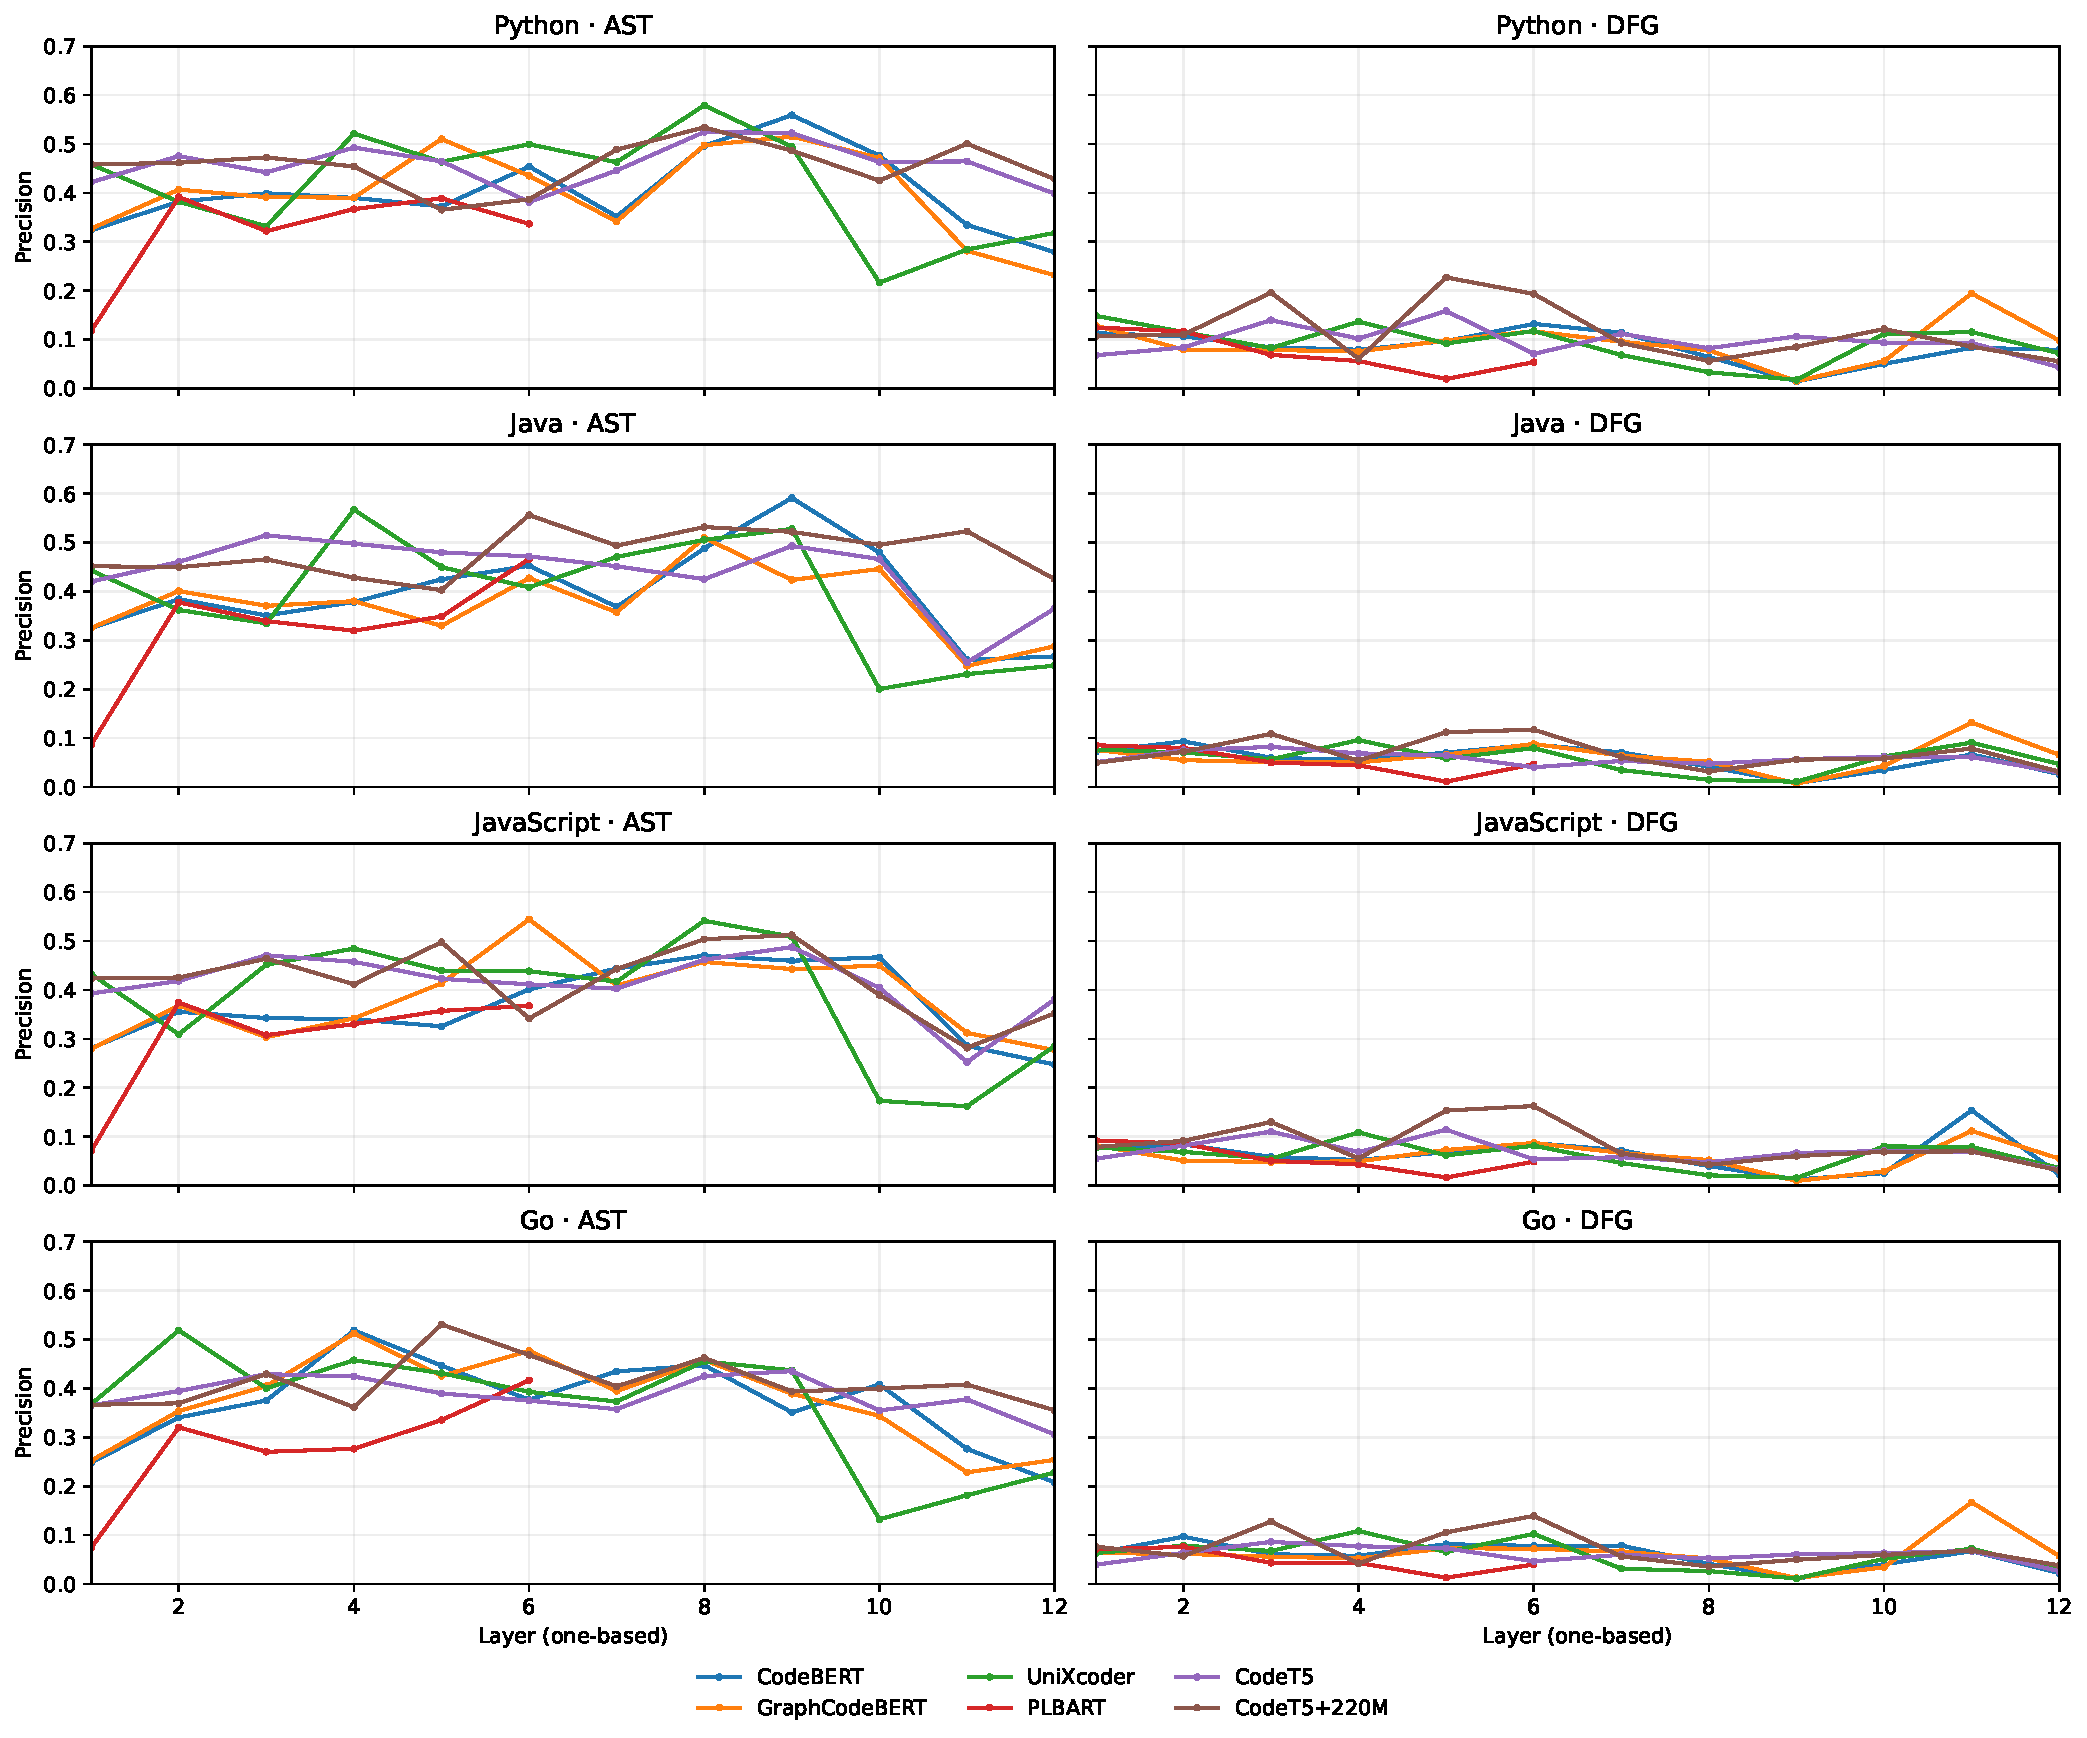
\includegraphics[width=\textwidth,height=0.78\textheight,keepaspectratio]{figures/figure7_precision_four_languages.pdf}
\caption{Four-language counterpart to the paper's Appendix Figure~7: precision of the same best-F-score attention heads against AST and DFG.}
\label{fig:precision}
\end{figure}

\section{Middle- and final-layer DirectProbe results}

The paper's Appendix~I also reports middle-layer DirectProbe results. Figure~\ref{fig:probe-layers} extends that comparison to layers 5, 9, and 12 for the same three models and five tasks in all four languages. The median across models at layer 12 is lower than at layer 5 in 19 of the 20 language--task groups; the sole exception is Go DFG, where the difference is about 0.003. The decrease is clearest for keyword--identifier siblings and both distance tasks. This qualifies the interpretation of Tables~\ref{tab:distance}--\ref{tab:dfg}: the last layer is the paper's reporting convention, but it is not generally the strongest layer for these probes. The figure reports overall test accuracy, unlike the per-label accuracies in the main tables.

\begin{figure}[p]
\centering
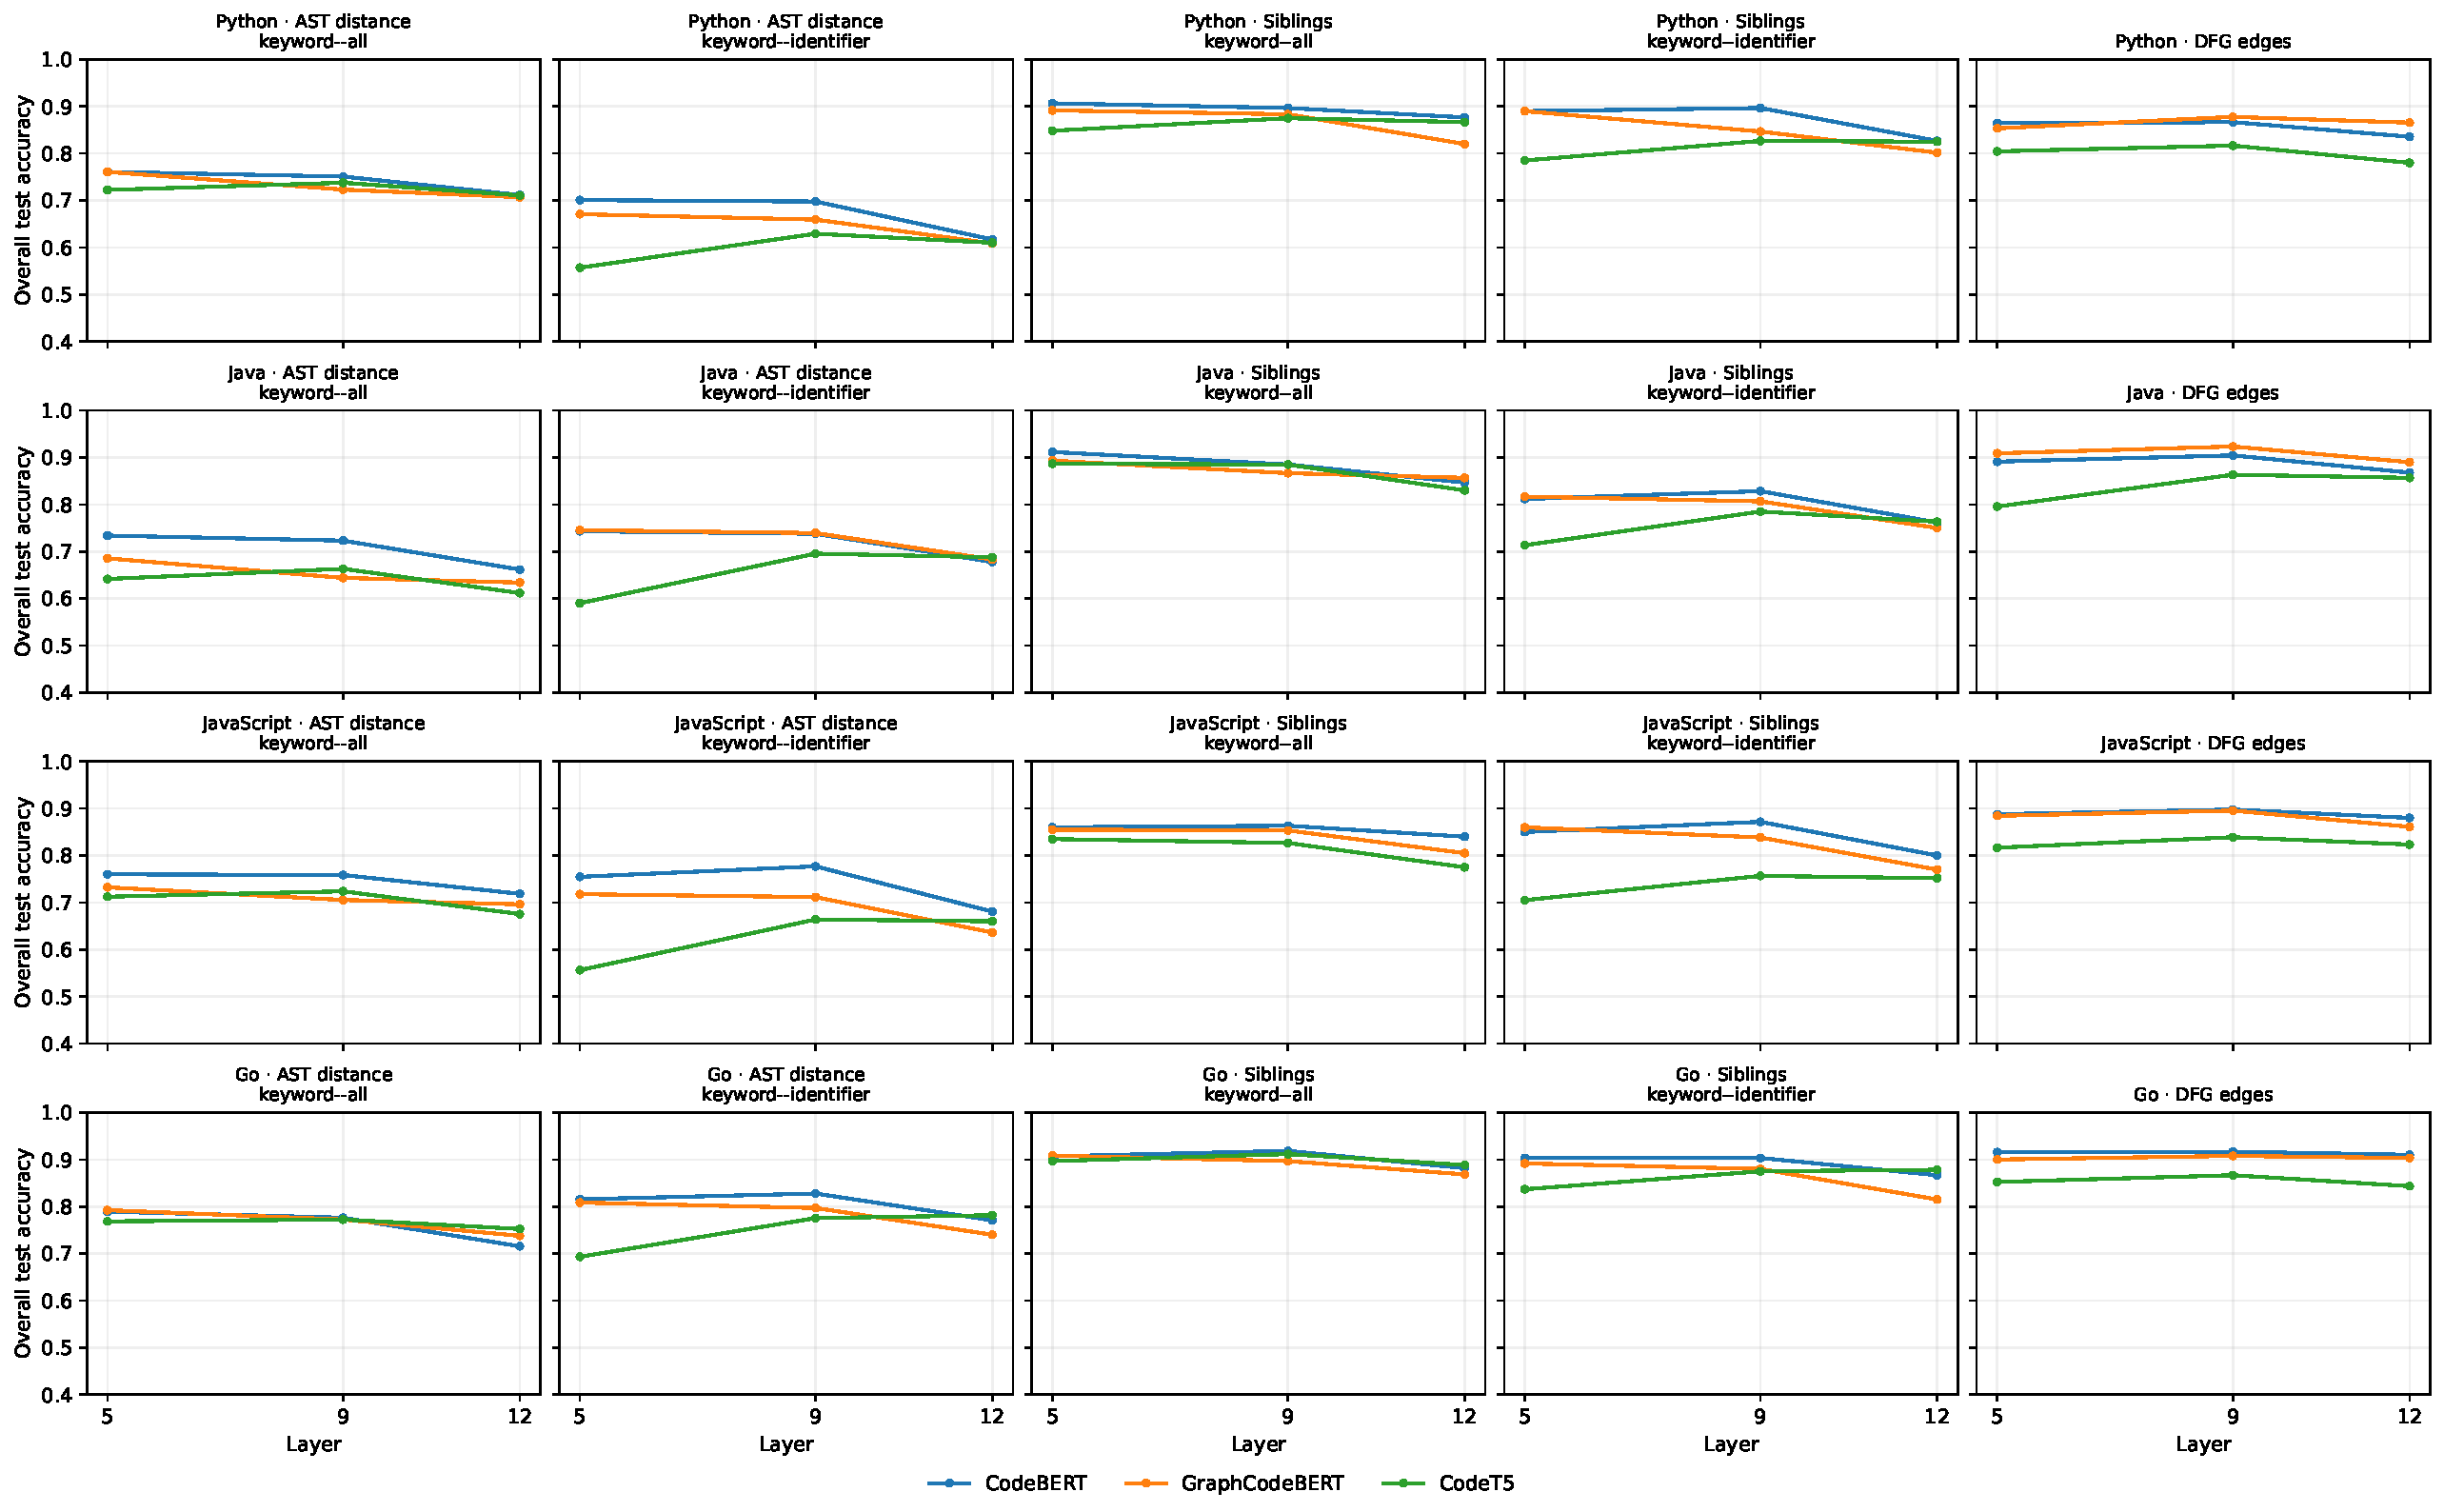
\includegraphics[width=\textwidth,height=0.8\textheight,keepaspectratio]{figures/appendix_probe_layers_four_languages.pdf}
\caption{Four-language comparison of DirectProbe overall test accuracy at layers 5, 9, and 12 for CodeBERT, GraphCodeBERT, and CodeT5, across the five paper tasks. Python is the original paper-repository reference; new languages are completed final-3000 runs.}
\label{fig:probe-layers}
\end{figure}

\end{document}
